\documentclass{report}
\textheight = 21cm % largo texto impreso
\textwidth = 16cm % ancho texto impreso
%\topmargin = -2cm % margen superior 3-2=1cm
\oddsidemargin = 0cm  % margen izquierdo 4.5-2=2.5cm
% Sangr\'ia=0mm
\parindent = 0mm
% Otros paquetes
\usepackage{amsmath,amssymb,amsfonts,latexsym}
\usepackage[T1]{fontenc} % fuentes adecuadas para salida
%\usepackage[latin1]{inputenc} % acentos,etc., desde el teclado
%\usepackage[utf8]{inputenc}
\usepackage{hyperref}
\usepackage{graphicx}
\usepackage{graphics}
\usepackage{verbatim}
\usepackage{pdfpages}
\usepackage{listings}
\usepackage{multimedia}
\usepackage{subcaption}
\usepackage[ruled,vlined,lined,linesnumbered]{algorithm2e}
\graphicspath{{imagenes/}}
%Paquete para escribir en otro idioma distinto del o ingl\'es. Este paquete traduce todos los textos est\'andar (“figure”,”chapter”,”section”,…) al idioma deseado:
\usepackage[spanish]{babel}
%Paquete para poder escribir los acentos de manera normal:
%\usepackage[latin1]{inputenc}
%\usepackage{amsmath}

\lstdefinestyle{customc}{
	belowcaptionskip=1\baselineskip,
	breaklines=true,
	frame=L,
	xleftmargin=\parindent,
	language=C,
	showstringspaces=false,
	basicstyle=\footnotesize\ttfamily,
	keywordstyle=\bfseries\color{green!40!black},
	commentstyle=\itshape\color{purple!40!black},
	identifierstyle=\color{blue},
	stringstyle=\color{orange},
}

\lstset{escapechar=@,style=customc}

%\usepackage{titlesec}
%\titleformat{\section}[frame]{\normalfont} %
%{\filright\footnotesize\enspace \thesection\enspace} %
%{8pt}{\Large\bfseries\filcenter} %
%-
%\titleformat{\chapter}[display]{\normalfont\Large\filcenter\sffamily} %
%{\titlerule[1pt] %\vspace{1pt}%
%	\titlerule
	%\vspace{1pc}%
%	\LARGE\MakeUppercase{\chaptertitlename} \thechapter}
%{1pc}
%{\titlerule
	%\vspace{1pc}%
%	\Huge}

%\usepackage[Bjornstrup]{fncychap}

%\AtBeginDocument{%\renewcommand\tablename{Tabla}} % Nombres para las tablas
%\renewcommand{\baselinestretch}{1.1} % espaciado 1.1
%\pagestyle{myheadings}
%\markright{\footnotesize \underline{Alc\'antara, Y. (2019) ``An\'alisis de soluciones de problemas seleccionados de la Final Mundial del ICPC 2019''}} % Encabezados simples
	
\usepackage{makeidx}
\makeindex

%\title{{\bf Informe de Pr\'actica Laboral}\\Identificaci\'on Semi-autom\'atica de Estenosis en Im\'agenes de Angiograf\'ia por Rayos-X} % Title
%
%\author{{\bf Estudiante}: Yuri \textsc{Alc\'antara Olivero}\\
%		{\bf Carrera}: Ciencia de la Computaci\'on\\
%		{\bf Facultad}: Ciencias Naturales y Exactas\\
%		Universidad de Oriente} % Author name

%\title{An\'alisis de soluciones de problemas seleccionados de la Final Mundial del ICPC 2019} % Title

%\author{Estudiante: Yuri \textsc{Alc\'antara Olivero}} % Author name
		
%\hyphenation{par-ti-cu-lar co-rres-pon-dien-te}

\begin{document}
\pagenumbering{roman}

\includepdf[pages=-]{portada}

%\maketitle % ++ the title, author and date


\setlength\parindent{0pt} % Removes all indentation from paragraphs

%\renewcommand{\labelenumi}{\alph{enumi}.} % Make numbering in the enumerate environment by letter rather than number (e.g. section 6)

\chapter*{Agradecimientos}
Agradezco a mi familia y a mi novia por el apoyo incondicional que siempre me brindaron.\\[0.2cm] 
A mis compa\~neros de equipo y a todas las personas que de alguna manera hicieron posible los resultados alcanzados.\\[0.2cm]
De manera especial a Pedro Rafael Reyes Terrero, la persona que me introdujo en el mundo de la programaci\'on.\\
\begin{flushright}
A todos, {\bf MUCHAS GRACIAS}.
\end{flushright}



%\hspace{1cm}\\[5cm]
%{\huge \textbf{Resumen}}\\[0.5cm]
\chapter*{Resumen}
La Competencia Internacional Universitaria ACM-ICPC es un concurso anual basado en equipos de programaci\'on. Esta es reconocida como una de las competencias m\'as antiguas y prestigiosas del mundo. Los equipos est\'an conformados por tres estudiantes y un entrenador.
Los estudiantes de la carrera de Ciencia de la Computaci\'on de la Universidad de Oriente participan todos los a\~nos en este concurso. Para obtener buenos resultados en estas competencias necesitan mucho tiempo de estudio independiente y preparaci\'on en temas de algoritmia y trabajo en equipo. Es por ello que en este trabajo se propone elaborar un solucionario de problemas seleccionados de la Final Mundial del ICPC 2019 para promover y motivar el entrenamiento de los estudiantes de la carrera de Ciencia de la Computaci\'on de la Universidad de Oriente.%\\[15,7 cm]

%\hspace{1cm}\\[5cm]
%{\huge\textbf{Abstract}}\\[0.5cm]
\chapter*{Abstract}
The ACM International Collegiate Programming Contest (ACM-ICPC) is a team-based annual competition known as one of the oldest and prestigious competitions in the world. The teams are conformed by three students and a coach. The students of Computer Science at Universidad de Oriente compete every year in this contest. To obtain good results in this kind of competitions, it is needed hard studies of algorithms and team-working. That is why we propose elaborating a solutionary of selected problems of the World Final ICPC 2019 to promote and motive the training of the students of Computer Science at Universidad de Oriente.

\tableofcontents 

%\pagenumbering{arabig}
%----------------------------------------------------------------------------------------
%	SECTION 1
%----------------------------------------------------------------------------------------
%\hspace{1cm} \\[21,7cm]
%{\huge \textbf{Introducci\'on}}\\[1cm]
\chapter*{Introducci\'on}
\addcontentsline{toc}{chapter}{Introducci\'on}
\pagenumbering{arabic}

La Asociaci\'on de Maquinaria Computacional\footnote{\hyperlink{ACM}{https://www.acm.org/}} (ACM, por sus siglas en ingl\'es) fundada en 1947, es una sociedad cient\'ifica y educativa relacionada con la Ciencia de la Computaci\'on. La ACM es una organizaci\'on de punta para los acad\'emicos y cient\'ificos interesados en esta \'area. Su lema es: ``Avanzar la Computaci\'on como Ciencia y Profesi\'on''. La ACM publica revistas y peri\'odicos cient\'ificos, adem\'as, patrocina variadas conferencias tales como SIGGRAPH\footnote{es una conferencia anual de Computaci\'on Gr\'afica auspiciada por la ACM-SIGGRAPH (Grupo Especial de Inter\'es en Gr\'aficos de Computadora y T\'ecnicas Interactivas.)\hyperlink{SIGGRAPH}{https://www.siggraph.org/}} y SIGCOMM\footnote{es una conferencia anual l\'ider en comunicaci\'on de datos y redes organizada por la ACM-SIGCOMM (Grupo Especial de Inter\'es en Comunicaciones de Datos)\hyperlink{SIGCOMM}{https://www.sigcomm.org/}}. Uno de los eventos m\'as importantes organizado por la ACM en el \'ambito universitario es la Competici\'on Internacional Universitaria ACM de Programaci\'on \footnote{\hyperlink{ACMICPC}{https://en.wikipedia.org/wiki/ACM\_International\_Collegiate\_Programming\_Contest}} (ACM-ICPC), la cual es reconocida como una de las competencias m\'as antiguas y prestigiosas del mundo.
La ACM-ICPC tuvo sus inicios en la Universidad A\&M de Texas en 1970. Al cabo de 7 a\~nos
pas\'o a ser una competici\'on con varias rondas clasificatorias. De 1977 a 1989, poco a poco se
fueron incluyendo m\'as universidades, compitiendo principalmente equipos de Estados Unidos y
Canad\'a. A partir de 1989 se convirti\'o en un concurso anual donde participan universidades de
todo el mundo, con la sede central ubicada en la Universidad de Baylor en Estados Unidos. Las
competiciones se desarrollan bajo el auspicio de la ACM y la colaboraci\'on de grandes empresas
de la industria inform\'atica. A estas competencias asisten equipos conformados por 3 estudiantes
y un entrenador, que es quien, fuera de competencia, se encarga de prepararlos y orientarlos
en cuanto al estudio de temas de programaci\'on, algoritmia y trabajo en equipo. Durante las
competencias los estudiantes disponen de una sola computadora para resolver alrededor de 12
problemas durante un periodo ininterrumpido, que puede ser de 4 a 5 horas, dependiendo del
nivel de la competencia. En los ciclos de competencias ACM-ICPC se realizan competencias
clasificatorias escalonadas, empezando en las universidades, y los mejores equipos avanzan a la
Competencia Regional. Luego se seleccionan los equipos ganadores de las competencias regionales y estos participan en la Final Mundial\footnote{https://icpc.baylor.edu/worldfinals/pdf/Factsheet.pdf}.\\

La Final Mundial tiene una duraci\'on de 5 horas, con alrededor de 12 problemas a resolver.
Cada equipo debe ser capaz de escribir un c\'odigo en alguno de los lenguajes de programaci\'on
permitidos (C, C++, Java, Python y Kotlin) para cada uno de los problemas que se ajuste
al tiempo de ejecuci\'on y la memoria requerida, y que debe ser correcto en todos los casos
de prueba previstos por los jueces. Las soluciones se juzgan de manera autom\'atica por un
sistema computacional que decide si la soluci\'on es correcta o no. Las soluciones incorrectas son
rechazadas y el equipo puede seguir intentando resolver el mismo problema. La puntuaci\'on de
cada equipo consiste de dos partes: cantidad de problemas resueltos y tiempo de penalizaci\'on,
en ese orden. Durante la competencia se muestra en tiempo real un ordenamiento de todos los
equipos que est\'an compitiendo seg\'un sus puntuaciones en el tiempo transcurrido, as\'i como las
respuestas que ha dado el jurado para todos los intentos de soluci\'on enviados\footnote{\hyperlink{quora}{https://www.quora.com/What-is-WA-RTE-CTE-and-TLE}}. Este standing
es visible tanto para los equipos como para el p\'ublico de la competencia.
En el ciclo de competencias ACM-ICPC 2018-2019, alrededor de 52000 estudiantes de m\'as de 3000 universidades
de 111 pa\'ises participaron en los distintos niveles. De estos, 405 estudiantes de 135 universidades
de alrededor de 40 pa\'ises, lograron clasificar a la Final Mundial 2019, celebrada en Porto, Portugal,
en el mes de abril. Este a\~no la competencia cont\'o con 11 problemas.
La Final Mundial del ACM-ICPC es la meta para la mayor\'ia de los estudiantes universitarios que participan en las competencias de programaci\'on competitiva. Cuba participa en estas
competencias desde el a\~no 2010. Poco a poco, el Movimiento de Programaci\'on Competitiva se
ha extendido a casi todas las universidades del pa\'is. Muchos estudiantes de la Universidad de Oriente, mayormente de la carrera de Ciencia de la Computaci\'on, participan en las competencias de
ACM-ICPC. La Universidad de Oriente clasific\'o por primera vez a una Final Mundial en el a\~no
2014, y ha logrado clasificar en 4 ocasiones m\'as (2015, 2016, 2018, 2019).
Obtener buenos resultados requiere de entrenamiento, estudio y de realizar muchas competencias, pero el curr\'iculo base y optativo de la carrera no es suficiente para lograr esta preparaci\'on, que en gran medida es garantizada por los entrenadores y el trabajo independiente de los
estudiantes interesados. Estas cuestiones fueron abordadas en un trabajo previo acerca de la Final Mundial ICPC 2018\cite{Aurora} pero la tendencia en estas competiciones es a ser cada vez m\'as exigentes. Por esta raz\'on los participantes se ven obligados a mantener una constante actualizaci\'on de los conocimientos en temas de programaci\'on competitiva y a resolver problemas cada vez m\'as complejos.\\[0.1cm]

Es por esto que se identific\'o como {\bf problema}:\\
{\it La carencia de habilidades en los estudiantes de la carrera de Ciencia de la Computaci\'on en
temas de Programaci\'on Competitiva.}\\[0.2cm]
Como consecuencia, se plante\'o la siguiente {\bf idea a defender}:\\
{\it La creaci\'on de un solucionario de problemas de la Final Mundial ICPC 2019, puede
favorecer el entrenamiento de los estudiantes de la carrera de Ciencia de la Computaci\'on de la
Universidad de Oriente que participan en competencias de Programaci\'on Competitiva.}\\[0.2cm]
Como {\bf objetivo general} de este trabajo se propuso:\\
{\it Resolver y proveer un solucionario detallado de problemas seleccionados de
la Final Mundial ICPC 2019.}\\
Para cumplir este objetivo se trazaron los siguientes {\bf objetivos espec\'ificos}:\\
\begin{enumerate}
	\item  Estudiar la teor\'ia necesaria para ser capaz de comprender y programar la soluci\'on de los
	problemas. 				
	\item Analizar la complejidad computacional de las soluciones propuestas.
	\item  Implementar la correcta soluci\'on de los problemas.
	\item Describir detalladamente las soluciones a los problemas. 
\end{enumerate} 

El resto del trabajo se estructura como sigue: dos cap\'itulos, conclusiones, recomendaciones y referencias bibliogr\'aficas. En el cap\'itulo \ref{chap:FundamentoTeorico} se exponen los fundamentos te\'oricos necesarios para la comprensi\'on de las soluciones a los problemas de la competencia. En cap\'itulo \ref{chap:Solucion}, se presenta la explicaci\'on y el c\'odigo de la soluci\'on de los problemas seleccionados. Finalmente son presentadas las conclusiones y las recomendaciones del trabajo. 

\chapter{Fundamentos Te\'oricos}
\label{chap:FundamentoTeorico}
En este cap\'itulo se abordan los temas fundamentales de Programaci\'on Competitiva necesarios para la correcta comprensi\'on de las soluciones de los problemas aqu\'i expuestas. Primero se introduce la Teor\'ia de Grafos, as\'i como algoritmos aplicados sobre estos. Luego se abordan algunas t\'ecnicas de Dise\~no y An\'alisis de Algoritmos. Tambi\'en se contempla el trabajo con cadenas y una de las estructuras m\'as usadas: Suffix Array. Finalmente se explica c\'omo se almacenan los n\'umeros en las computadoras, con esa informaci\'on se calcula la cantidad de bits que un programa utiliza durante su ejecuci\'on. Esto se tiene en cuenta a la hora de dise\~nar soluciones que cumplan con los l\'imites de memoria establecidos en la Final Mundial del ICPC.

\section{Teor\'ia de Grafos}
A continuaci\'on se muestran los conceptos y definiciones de grafos dirigidos y no dirigidos, con
peso, con ciclos, componentes conexas, entre otros \cite{Cormen}\cite{Halim}\cite{Graph1}\cite{Graph2}. Adem\'as se explican dos algoritmos
de recorrido en grafos.\\\\
{\bf Definici\'on} 1. Un grafo G es una estructura compuesta por un conjunto V de elementos llamados nodos, y un conjunto E de pares de nodos relacionados llamados aristas.\\\\
{\bf Definici\'on} 2. Un grafo se denomina dirigido cuando las relaciones entre los nodos son unidireccionales, y se denomina no dirigido cuando las relaciones son bidireccionales.\\\\
{\bf Definici\'on} 3. Un grafo es pesado cuando sus aristas tienen asociadas un valor real.\\\\
{\bf Definici\'on} 4. Se denota la arista entre el nodo u y el nodo v como (u, v) en un grafo no dirigido
y en un grafo dirigido se denota u $\rightarrow$ v.\\\\
{\bf Definici\'on} 5. En un grafo no dirigido la arista (u, v) se dice que incide en u y en v.\\\\
{\bf Definici\'on} 6. Se denomina lazo a una arista de un grafo no dirigido que se expresa como (u, u).\\\\
{\bf Definici\'on} 7. En un grafo no dirigido sin lazos se llama grado de un nodo v, y se denota por
g(v), a la cantidad de aristas que inciden en \'el.\\\\
{\bf Definici\'on} 8. Un camino es una lista de nodos tal que cada nodo est\'a conectado mediante una
arista al siguiente nodo de la lista. La longitud del camino es la suma de los pesos de las aristas
de este.\\\\
{\bf Definici\'on} 9. Un ciclo es un camino que no tiene nodos repetidos, a excepci\'on del primer nodo
que coincide con el \'ultimo.\\\\
{\bf Definici\'on} 10. Un grafo dirigido ac\'iclico (DAG) es un grafo con aristas dirigidas que no
contiene ciclos.\\\\
{\bf Definici\'on} 11. Se llama conexo a un grafo no dirigido que cumple que entre dos cualesquiera
de sus v\'ertices existe un camino que los une.\\\\
{\bf Definici\'on} 12. Sea G = (V, E) un grafo. Se dice que el grafo $G' = (V', E')$ es un subgrafo de
G si y solo si $V' \subseteq V $y $E' \subseteq E $ y los extremos de las aristas que contiene $E'$ pertenecen al
conjunto $V'$.\\\\
{\bf Definici\'on} 13. Se llama componente conexo de un grafo no dirigido a todo subgrafo conexo
maximal del grafo, esto es, que no est\'a contenido en ning\'un otro subgrafo conexo del grafo.\\\\
{\bf Definici\'on} 14. Un \'arbol es un grafo conexo que no contiene ciclos.\\\\
{\large Recorridos en Grafos}\\
Los algoritmos de recorridos en grafos son aquellos que permiten visitar todos los nodos de
un grafo seg\'un la preferencia que se desee. Los dos recorridos empleados con mayor frecuencia
son b\'usqueda a lo ancho y b\'usqueda en profundidad.\\
{\bf B\'usqueda a lo ancho primero (BFS)}\\
Dado un grafo G = (V, E) y un v\'ertice v, el algoritmo explora sistem\'aticamente los v\'ertices
de G para descubrir los v\'ertices que son alcanzables a partir de v \cite{Cormen}. Este algoritmo computa
la menor distancia del nodo inicial v a todo v\'ertice alcanzable. A continuaci\'on se muestra un
seudoc\'odigo del mismo.

\begin{algorithm}[H] % H = forzar est\'a posici\'on
	\caption{BFS(G,v)}\label{ML:Algorithm1}
	\SetAlgoLined
	\LinesNumbered
	\SetAlgoVlined
	Q es una cola(FIFO)\\
	a\~nadir v a Q\\
	marcar v como visitado\\
	{\bf Mientras} Q no est\'e vac\'ia {\bf Hacer}\\
	\hspace{1cm}Extraer t de Q\\
	\hspace{1cm}{\bf Para todo nodo} u adyacente de t no visitado {\bf Hacer}\\
	\hspace{2cm}a\~nadir u a Q\\
	\hspace{2cm}marcar u como visitado\\
	\hspace{1cm}{\bf Fin Para}\\
	{\bf Fin Mientras}\\

\end{algorithm}
\hspace{1cm}\\

{\bf B\'usqueda en profundidad primero (DFS)}\\
Dado un grafo G = (V, E) y un v\'ertice escogido v, el algoritmo recursivamente explora lo
m\'as profundo que le sea posible\cite{Cormen}. Este se plantea en el siguiente seudoc\'odigo:\\

\begin{algorithm}[H] % H = forzar est\'a posici\'on
	\caption{DFS(G,v)}\label{ML:Algorithm2}
	\SetAlgoLined
	\LinesNumbered
	\SetAlgoVlined
	marcar v como visitado\\
    {\bf Para todo nodo} u adyacente de v no visitado {\bf Hacer}\\
	\hspace{1cm}DFS(G,u)\\
   {\bf Fin Para}\\
	
\end{algorithm}
\hspace{1cm}\\


Ambos algoritmos tiene una complejidad espacial de O(|V| + |E|) si G es conexo, sino, la
complejidad es de acuerdo a la cantidad de v\'ertices y la cantidad de aristas de la componente
conexa a la que pertenece el nodo v. Estos permiten calcular los nodos que est\'an en la misma
componente conexa de un nodo v seleccionado.

\section{T\'ecnicas de Dise\~no y An\'alisis de Algoritmos}
En esta secci\'on se presentan dos T\'ecnicas de Dise\~no de Algoritmos: Programaci\'on Din\'amica
y Estrategia Greedy.

\subsection{Programaci\'on Din\'amica}
La t\'ecnica de Programaci\'on Din\'amica consiste en solucionar un problema combinando las
soluciones de subproblemas y se utiliza cuando estos subproblemas no son disjuntos \cite{Cormen}\cite{Halim}\cite{DP1}. Soluciona
problemas de optimizaci\'on, donde el problema tiene varias soluciones y se desea saber cu\'al es
la \'optima de acuerdo a un criterio espec\'ifico. Cuando se utiliza un algoritmo de Programaci\'on
Din\'amica se siguen los siguientes pasos:
\begin{enumerate}
\item[1-] Caracterizar la estructura de la soluci\'on \'optima.
\item[2-] Recursivamente definir el valor de la soluci\'on \'optima.
\item[3-] Calcular el valor de las soluciones \'optimas.
\item[4-] Construir la soluci\'on \'optima a partir de la informaci\'on ya calculada.
\end{enumerate}

\subsection{Algoritmos Golosos ( Greedy )}
Los algoritmos Greedy siempre escogen la mejor soluci\'on de manera local con la suposici\'on de
que esta les llevar\'a a la soluci\'on global\cite{Cormen}\cite{Halim}. Estos algoritmos no siempre calculan el \'optimo global,
pero en muchos casos s\'i lo hacen. Para utilizarlos es necesario demostrar que en la soluci\'on se
pueden tomar las decisiones greedy y se alcanza el valor \'optimo. La estrategia Greedy tiene la
ventaja de que resuelve un problema mucho m\'as r\'apido que utilizando Programaci\'on Din\'amica.

\section{Trabajo con cadenas}
Uno de las m\'as simples y naturales formas de representaci\'on de la informaci\'on son los textos. Este tipo de datos se caracteriza por el hecho de que puede ser escrito como una secuencia de caracteres. Los algoritmos de texto se utilizan en muchas \'areas de la ciencia y en el procesamiento de informaci\'on. En biolog\'ia por ejemplo los algoritmos de texto contribuyen al estudio de secuencias moleculares. El problema b\'asico en esta \'area es el ``pattern matching'' como se conoce en ingl\'es, consiste en encontrar coincidencias de patrones en un texto determinado.\cite{TextAlgorithm}\cite{Halim}.\\
\subsection{Suffix Array}
Existe una idea simple y astuta de trabajar con los sufijos de un texto: tenerlos ordenados de manera creciente lexicogr\'aficamente para realizar operaciones sobre ellos de manera eficiente. La implementaci\'on de esta idea nos lleva a una estructura de datos llamada Suffix Array.\cite{TextAlgorithm}.\\
El primer m\'etodo en el que se puede pensar para ordenar sufijos es usar un algoritmo est\'andar de ordenamiento O($N \;log\; N$). Como la comparaci\'on entre sufijos se realiza en O($N$), la complejidad final ser\'ia O($N^2 \;log\;N$). Existe un algoritmo relativamente sencillo para realizar este ordenamiento en O($N\;log\;N$). El algoritmo est\'a basado principalmente en la idea de ordenar los sufijos teniendo en cuenta sus prefijos de tama\~no $2^k$\cite{SuffixArray}\cite{SuffixArray1}.
\section{Almacenamiento de los n\'umeros en las computadoras actuales}
A continuaci\'on se muestra una tabla de cu\'anto espacio ocupan los tipos de datos utilizados
en un programa:

	\begin{table}[h!]
		\centering
		\begin{tabular}{|l|c|c|} \hline
			{\bf Nombre} & {\bf Tama\~no en bits} & {\bf Rango que puede representar} \\\hline
			Char  & 8 & $-2^7 \;a\;2^7 - 1$\\\hline
			Short  & 16  &$-2^{15} \;a\;2^{15} - 1$\\\hline
			Unsigned Short  & 16  &$0 \;a\;2^{16} - 1$\\\hline
			Int  & 32  &$-2^{31} \;a\;2^{31} - 1$\\\hline
			Unsigned Int  & 32  &$0 \;a\;2^{32} - 1$\\\hline
			Long  & 32 &$-2^{31} \;a\;2^{31} - 1$\\\hline
			Unsigned Long  & 32  &$0 \;a\;2^{32} - 1$\\\hline
			Long Long  & 64  &$-2^{63} \;a\;2^{63} - 1$\\\hline
			Unsigend Long Long  & 64  &$0 \;a\;2^{64} - 1$\\\hline
			Float & 32  &$−3.4 \cdot 10^{38}\; a \;3.4 \cdot 10^{38}$\\\hline
			Double & 64  &$\pm 5.0 \cdot 10^{−324} \;a\; \pm 1.7 \cdot 10^{308}$\\\hline
		\end{tabular}
		\caption{Tipos de datos.}
		\label{TiposDatos}
	\end{table}
	\hspace{1cm}\\
	Los n\'umeros decimales se guardan de una manera espacial, tienen por separado mantisa(m),
	exponente(e) y signo(s). A partir de estos 3 valores el n\'umero almacenado es igual a $s \cdot m \cdot 2^e$.
	
	\begin{table}[h!]
		\centering
		\begin{tabular}{|l|c|c|c|} \hline
			{\bf Nombre} & {\bf Signo} & {\bf Exponente} & {\bf Mantisa}\\\hline
			float  & 1 & 8 & 23\\\hline
			Short  & 1  & 11 & 52\\\hline
		\end{tabular}
		\caption{Representaci\'on de n\'umeros decimales}
		\label{Decimales}
	\end{table}
	\hspace{1cm}\\

En la competencia Final Mundial ICPC 2019, los problemas ten\'ian un l\'imite de un 1gb de
memoria, lo cual es alrededor de $8 \cdot 10^9$ bits. Es decir, el c\'odigo que solucione los problemas no
debe almacenar m\'as de $c \cdot 8 \cdot 10^9$ bits, donde c es una constante.
En cuanto al tiempo de ejecuci\'on, un segundo en el jurado online utilizado en la competencia,
equivale a $10^8$ operaciones, por lo tanto, la cantidad de operaciones permisibles para cada
problema es $c \cdot s \cdot 10^8$, donde c es una constante y s es la cantidad de segundos que exige el
problema en cuesti\'on.

\chapter{Soluci\'on de los problemas}
\label{chap:Solucion}
En este cap\'itulo se presenta la soluci\'on de los 6 problemas escogidos de la Final Mundial
del ICPC 2019. De cada problema se muestra su enunciado, tal y como es ofrecido durante la
competencia(en idioma ingl\'es), a continuaci\'on una descripci\'on m\'as formal del mismo en espa\~nol,
donde se  	exponen solo los hechos importantes necesarios para solucionar el problema, luego se
expone la soluci\'on incluyendo el an\'alisis de la complejidad computacional\cite{Knuth}\cite{Complejidad1}\cite{Complejidad2} en cada caso y finalmente el c\'odigo que ha sido aceptado en el juez online Kattis\footnote{\hyperlink{Kattis}{https://icpc.kattis.com/problems}}, que
contiene los problemas analizados.

\section{Problema A. Azulejos}
Ceramic artists Maria and Jo\~ao are opening a small azulejo store in Porto. Azulejos are the beautiful ceramic tiles for which Portugal is famous. Maria and Jo\~ao
want to create an attractive window display, but, due to limited space in their
shop, they must arrange their tile samples in two rows on a single shelf. Each of
Jo\~ao's tiles has exactly one of Maria's tiles in front of it and each of Maria's tiles
has exactly one of Jo\~ao's tiles behind it. These hand-crafted tiles are of many
different sizes, and it is important that each tile in the back row is taller than the
tile in front of it so that both are visible to passers-by. For the convenience of
shoppers, tiles in each row are arranged in non-decreasing order of price from
left to right. Tiles of the same price may be arranged in any order subject to the
visibility condition stated above.
Your task is to find an ordering of the tiles in each row that satisfies these constraints, or determine that
no such ordering exists.\\

\begin{figure}[h]
	\begin{center}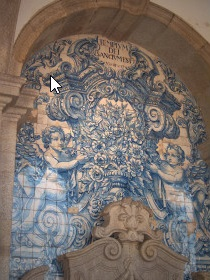
\includegraphics[scale=0.45]{Azulejos}\end{center}
	\caption{Azulejo in the cathedral of Porto.}	
	\label{Azulejos}
\end{figure}

{\bf Input}\\
The first line of input contains an integer $n\; (1 \leq n \leq 5 \cdot 10^5)$, the number of tiles in each row. The next
four lines contain n integers each; the first pair of lines represents the back row of tiles and the second
pair of lines represents the front row. Tiles in each row are numbered from 1 to n according to their
ordering in the input. The first line in each pair contains n integers $p_1, \ldots, p_n (1 \leq p_i \leq 10^9$ for each
i), where $p_i$ is the price of tile number i in that row. The second line in each pair contains n integers
$h_1,\ldots , h_n \;(1 \leq h_i \leq 10^9$ for each i), where h i is the height of tile number i in that row.\\
{\bf Output}\\
If there is a valid ordering, output it as two lines of n integers, each consisting of a permutation of the
tile numbers from 1 to n. The first line represents the ordering of the tiles in the back row and the second
represents the ordering of the tiles in the front row. If more than one pair of permutations satisfies the
constraints, any such pair will be accepted. If no ordering exists, output {\it impossible}.
\subsection{Descripci\'on}
Dos artistas de la cer\'amica Joao y Mar\'ia poseen una tienda donde venden azulejos. Por limitaciones de espacio en la tienda ellos deben colocar los azulejos en dos filas, una con los azulejos de Joao y otra con los de Mar\'ia. Cada azulejo de Joao tiene exactamente un azulejo de Mar\'ia en frente y cada uno de los de Mar\'ia tiene uno de los de Joao detr\'as. Los azulejos tienen distintas alturas por lo que es importante que cada azulejo de Joao tenga una altura estrictamente mayor que el de Mar\'ia colocado en frente para que se pueda ver. Adem\'as, para la conveniencia de los compradores los azulejos deben estar colocados de izquierda a derecha en orden no decreciente considerando los precios.\\

B\'asicamente contamos con dos filas de N azulejos cada una, donde cada azulejo tiene un precio $(p_i)$ y una altura $(h_i)$ determinada. Llamemos a las filas A (azulejos de Joao) y B (azulejos de Mar\'ia). La descripci\'on del problema nos indica que despu\'es de ordenar cada una de las filas, la altura del kth azulejo de la fila A debe ser estrictamente mayor que la del kth de la fila B. Adicionalmente se requiere que los azulejos est\'en ordenados de manera no decreciente con respecto a los precios. Se nos pide encontrar un orden para cada fila que cumpla con las restricciones mencionadas anteriormente o determinar que dicho orden no existe.\\

L\'imites\\
$N \leq 500000$\\
$1 \leq p_i, h_i <=10^6$\\
Tiempo L\'imite: 12 segundos\\

\subsection{Soluci\'on}
La soluci\'on de este problema es de naturaleza golosa pero adem\'as requiere de trabajo con estructuras de datos para garantizar una soluci\'on que cumpla con el l\'imite de tiempo.\\

Al ordenar las filas de manera no decreciente por el precio, los azulejos de igual precio constituyen un intervalo continuo dentro de la fila. Estos a su vez son los que pueden intercambiar posiciones entre ellos dentro del orden determinado.\\ 
Sea IA el conjunto de todos los azulejos con el menor precio de la fila A e IB el conjunto de todos los azulejos con el menor precio de la fila B,
asumamos que $|IA|\leq|IB|$ sin perdida de generalidad, entonces todo $X \in IA$ debe emparejarse de manera obligatoria con alg\'un $Y\in IB$ y viceversa en caso de que $|IB|\leq|IA|$. Una vez emparejados dos elementos estos pasan a ser parte de la soluci\'on parcial y dejan de ser considerados, as\'i pasamos a resolver el mismo problema del principio con los azulejos restantes. Si en alg\'un momento no podemos emparejar uno de los elementos entonces determinamos que el orden buscado no existe. El problema ahora se reduce a elegir con quien emparejar cada elemento y es aqu\'i donde se toma la decisi\'on golosa de manera acertada.

Si |IA|<=|IB|\\ 
Escogemos un $X \in IA$, sea X.h su altura, debemos emparejar a X con un $Y \in IB$, tal que Y.h < X.h y ($\forall Z \in IB$ con Z.h < X.h y $Y.h \geq Z.h$). O sea debemos emparejar el elemento de IA con el de mayor altura de IB que pueda ser emparejado.\\ 
En otro caso(|IB|<|IA|)\\
Escogemos un $X \in IB$, sea X.h su altura, debemos emparejar a X con un $Y \in IA$, tal que Y.h > X.h y ($\forall Z \in IA$ con Z.h > X.h y $Y.h \leq Z.h$). Emparejar el elemento de IB con el de menor altura de IA que pueda ser emparejado.\\
En cada uno de los casos se trata de dejar los elementos m\'as convenientes para decisiones futuras garantizando encontrar una soluci\'on en caso de que exista.
Para implementar el algoritmo de manera eficiente debemos emplear una estructura de datos que nos permita hacer b\'usqueda binaria, pudiendo insertar y eliminar elementos con una complejidad logar\'itmica(Ej: std::multiset).
En este algoritmo cada elemento de las filas es insertado y eliminado de la estructura anteriormente descrita exactamente una vez por lo que se realizan $2\cdot(N\; log \;N) + N\; log\; N$ por la b\'usqueda binaria para cada emparejamiento. De aqu\'i se concluye que la complejidad algor\'itmica de esta soluci\'on es O(N log N). En el peor caso se realizan $27\cdot 10^6$ operaciones, menor que las $12 \cdot 10^8$ permisibles seg\'un el l\'imite de tiempo establecido para el problema. La soluci\'on tiene complejidad espacial $O(N)$, en el peor caso almacena $5\cdot 10^5 \cdot 4\; bytes$, menor que los $10^9 \;bytes$ permitidos.

\subsection{C\'odigo}
\begin{lstlisting}[language=C++]
#include <bits/stdc++.h>
using namespace std;

const int MAXN=5e5+5;
typedef pair<int,int>par;
struct azulejos
{
	int p,h,id;
	azulejos()
	{
		p=0,h=0,id=0;
	}
	bool operator < (const azulejos &a)const
	{
		return p < a.p;
	}
};
azulejos A1[MAXN],A2[MAXN];
multiset<par>MS1,MS2;
multiset<par>::iterator it1,it2;
vector<int>sol1,sol2;
bool Impossible=false;;

void proccess()
{
	if(MS1.size()<=MS2.size())
	{
		it1=MS1.begin();
		it2=MS2.lower_bound(par(it1->first,0));
		if(it2==MS2.begin())
		{
			Impossible=true;
			return;
		}
		it2--;
		sol1.push_back(it1->second);
		sol2.push_back(it2->second);
		MS1.erase(it1);
		MS2.erase(it2);
	}
	else
	{
		it2=MS2.begin();
		it1=MS1.upper_bound(par(it2->first,1<<30));
		if(it1==MS1.end())
		{
			Impossible=true;
			return;
		}
		sol1.push_back(it1->second);
		sol2.push_back(it2->second);
		MS1.erase(it1);
		MS2.erase(it2);
	}
}

int main()
{
	cin.tie(0);
	ios_base::sync_with_stdio(0);
	
	int N;
	cin >> N;
	
	for(int i=1; i<=N; i++)
	cin >> A1[i].p;
	for(int i=1; i<=N; i++)
	cin >> A1[i].h,A1[i].id=i;
	
	for(int i=1; i<=N; i++)
	cin >> A2[i].p;
	for(int i=1; i<=N; i++)
	cin >> A2[i].h,A2[i].id=i;
	
	sort(A1+1,A1+N+1);
	sort(A2+1,A2+N+1);
	
	int p1=1,p2=1;
	
	while(p1<=N || p2<=N)
	{
		if(MS1.empty())
		{
			int paux=p1;
			while(p1<=N && A1[paux].p==A1[p1].p)
			MS1.insert(par(A1[p1].h,A1[p1].id)),p1++;
		}
		if(MS2.empty())
		{
			int paux=p2;
			while(p2<=N && A2[paux].p==A2[p2].p)
			MS2.insert(par(A2[p2].h,A2[p2].id)),p2++;
		}
		
		proccess();
		if(Impossible)
		{
			cout << "impossible\n";
			return 0;
		}
		
	}
	
	while(!MS1.empty() && !MS2.empty())
	{
		proccess();
		if(Impossible)
		{
			cout << "impossible\n";
			return 0;
		}
	}
	cout << sol1[0];
	for(int i=1; i<N; i++)
	cout << ' ' << sol1[i];
	cout << '\n' << sol2[0];
	for(int i=1; i<N; i++)
	cout << ' ' << sol2[i];
	cout << '\n';
	
	return 0;
}

\end{lstlisting}
\section{Problema B. Beautiful Bridges}
What connects us all? Well, it is often bridges. Since ancient times, people have been building bridges for roads, for
trains, for pedestrians, and as aqueducts to transport water. It
is humanity's way of not taking inconvenient geography for an
answer.
The company Arch Bridges Construction (ABC) specializes
in-you guessed it-the construction of arch bridges. This
classical style of bridge is supported by pillars that extend
from the ground below the bridge. Arches between pillars distribute the bridge's weight onto the adjacent pillars.
The bridges built by ABC often have pillars spaced at irregular intervals. For aesthetic reasons, ABC's
bridges always have semicircular arches, as illustrated in Figure \ref{Bridge}. However, while a bridge arch can
touch the ground, it cannot extend below the ground. This makes some pillar placements impossible.\\
\begin{figure}[h]
	\begin{center}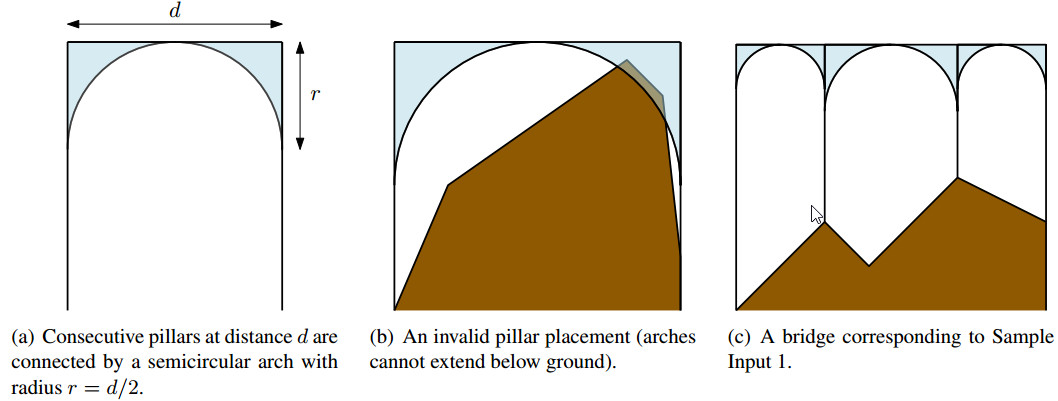
\includegraphics[scale=0.45]{Bridge}\end{center}
	\caption{Bridge example.}	
	\label{Bridge}
\end{figure}
Given a ground profile and a desired bridge height h, there are usually many ways of building an
arch bridge. We model the ground profile as a piecewise-linear function described by n key points
$(x_1,y_1), (x_2,y_2),\ldots, (x_n,y_n)$, where the x-coordinate of a point is the position along the bridge, and
the y-coordinate is the elevation of the ground above sea level at this position along the bridge. The first
and last pillars must be built at the first and last key points, and any intermediate pillars can be built only
at these key points. The cost of a bridge is the cost of its pillars (which is proportional to their heights)
plus the cost of its arches (which is proportional to the amount of material used). So a bridge with k
pillars of heights $h_1,\dots,h_k$ that are separated by horizontal distances $d_1,\ldots,d_{k−1}$ has a total cost of:
\begin{equation}
\alpha \cdot \sum_{i=1}^{k}\;h_i + \beta \cdot \sum_{i=1}^{k-1}\; {d_i}^2
\end{equation}
for some given constants $\alpha\; and\; \beta$. ABC wants to construct each bridge at the lowest possible cost.\\
{\bf Input}\\
The first line of input contains four integers n, h, $\alpha, \;and\; \beta$, where n $(2 \leq n \leq 10^4)$ is the number of
points describing the ground profile, h $(1 \leq h \leq 10^5)$ is the desired height of the bridge above sea level,
and $\alpha, \beta (1 \leq \alpha, \beta \leq 10^4)$ are the cost factors as described earlier. Then follow n lines, the ith of which
contains two integers $x_i, y_i (0 ≤ x_1 < x_2 < \ldots < x_n \leq 10^5 \;and\; 0 \leq y_i < h)$, describing the ground
profile.\\
{\bf Output}\\
Output the minimum cost of building a bridge from horizontal position $x_1\; to\; x_n$ at height h above sea
level. If it is impossible to build any such bridge, output {\it impossible}.\\
\subsection{Descripci\'on}
En el problema nos hablan de una empresa dedicada a la construcci\'on de puentes. Los puentes son soportados por pilares que se extienden desde la tierra hasta la parte inferior del puente. Los puentes tienen arcos en forma de semic\'irculo que van de un pilar al otro siguiente. El relieve debajo del puente es irregular lo que provoca que la colocaci\'on de algunos pilares sea imposible para una altura fija del puente (ver fig\ref{Bridge}). El relieve se modela con funciones lineales entre pares consecutivos de puntos $(x_1,y_1),\ldots,(x_n,y_n)$ donde $x_i$ representa una posici\'on a los largo del puente y $y_i$ la elevaci\'on sobre el nivel del mar de la tierra en ese punto. Los pilares solo pueden construirse en uno de estos puntos. De manera formal el costo de un puente con $K$ pilares con alturas $h_1,\ldots, h_k$ que est\'an separados por distancia horizontales $d_1,\ldots,d_{k-1}$ es:\\
\begin{equation}
\displaystyle{\alpha \cdot \sum_{i=1}^{k} + \beta \cdot \sum_{i=1}^{k-1} {d_i}^2}
\end{equation}
Las variables $\alpha$ y $\beta$ son constantes predefinidas. Se nos pide construir el puente con el menor costo posible que cumpla las restricciones descritas o determinar que es imposible construir uno.\\
L\'imites\\
$(2 \leq n \leq 10^4)$\\
$(1 \leq h \leq 10^5)$\\
$(1 \leq \alpha, \beta \leq 10^4)$\\
$(0 ≤ x_1 < x_2 < \ldots < x_n \leq 10^5 \;and\; 0 \leq y_i < h)$\\
Tiempo L\'imite: 10 segundos\\

\subsection{Soluci\'on}
Este problema tiene una soluci\'on est\'andar con programaci\'on din\'amica: La idea es calcular el mejor costo de cubrir los $i$ primeros puntos por supuesto con un pilar en el punto i. Luego consideramos todos los puntos $j < i$ para construir un arco de $j$ a $i$ si es v\'alido, de esa manera actualizamos el costo hasta $i$ con el costo hasta $j$ m\'as el costo del arco entre $i$ y $j$.\\
\begin{algorithm}[H] % H = forzar est\'a posici\'on
	\caption{MenorCosto(N,H,A,B,X,Y)}\label{ML:Algorithm3}
	\SetAlgoLined
	\LinesNumbered
	\SetAlgoVlined
	DP es un arreglo de enteros\\
	${DP}_1 = A \cdot (H - Y_1)$\\
	{\bf Para Cada}$\;2 \leq i \leq N$ {\bf Hacer}\\
	\hspace{1cm} $DP_i = Infinito$\\
	{\bf Fin Para}\\
	{\bf Para Cada}$\;1 \leq i \leq N$ {\bf Hacer}\\
	\hspace{1cm}{\bf Para Cada}$\;1 \leq j < i$ {\bf Hacer}\\
	\hspace{2cm}{\bf Si} ArcoValido(j,i) {\bf Hacer}\\ 
	\hspace{3cm}$DP_i = min(DP_i,\; DP_j + A\cdot(H-Y_i) + B\cdot{(X_j-X_i)}^2)$\\
	\hspace{2cm}{\bf Fin Si}\\
	\hspace{1cm}{\bf Fin Para}\\
	{\bf Fin Para}\\

\end{algorithm}
\hspace{1cm}\\
Comprobar si un arco es v\'alido se puede hacer de manera trivial en O(N). Supongamos que se construye un arco entre las posiciones $i$ y $j$, sea $d$ la distancia entre los pilares, el arco  puede ser descrito con la ecuaci\'on de la circunferencia de centro ($(X_j + X_i)/2$, $H - \frac{d}{2}$) y radio $\frac{d}{2}$. As\'i para un punto cualquiera ($X_k$, $Y_k$) con $i\leq k\leq j$ se puede evaluar la $x$ en la ecuaci\'on de la circunferencia y comparar la $y$ obtenida con la $y$ del punto. Lamentablemente realizar esta comprobaci\'on en O(N) implica que la complejidad del algoritmo total sea O($N^3$) lo cual es muy lento para satisfacer los l\'imites de tiempo. Para mejorar la soluci\'on se podr\'ia precalcular si un arco de $i$ a $j$ es v\'alido o no, al responder esta interrogante en O(1) la soluci\'on ser\'ia O($N^2$), aceptable para este problema. Por supuesto el prec\'alculo debe ser O($N^2$) o inferior para que tenga sentido esta soluci\'on.\\
La primera observaci\'on es que si fijamos un pilar en la posici\'on i y tratamos de extender un arco hacia la derecha, la mitad izquierda del arco necesita cada vez m\'as espacio. Esto indica que para una distancia $d$ del arco, si un punto ($X_k$, $Y_k$)de la tierra est\'a sobre o por encima de la mitad izquierda del arco entonces para una distancia mayor que d tambi\'en lo estar\'a. De la misma manera si un punto est\'a por debajo de la parte izquierda del arco para una distancia d tambi\'en lo estar\'a para una menor. Usando esta idea se puede calcular para cada punto $i$ el arco m\'as largo hacia la derecha que se puede construir sin que su mitad izquierda toque la tierra. Lo podemos hacer en O($N^2$) fijando un puntero al final que indica hasta donde se puede construir el arco y para cada punto a la derecha corremos el puntero hacia la izquierda mientras sea necesario. Con ese an\'alisis se puede realizar el mismo c\'alculo hacia la izquierda, o sea determinar la posici\'on m\'as a la izquierda $j$ que permita construir un arco del punto $j$ al $i$ sin que la mitad derecha del arco toque la tierra. Con estas dos informaciones se puede comprobar en O(1) si un arco desde un punto $l$ hasta uno $r$ es v\'alido. La complejidad algor\'itmica total de la soluci\'on en O($N^2$), en el peor caso se realizan $10^8$ operaciones, menor que las $10 \cdot 10^8$ permisibles seg\'un el l\'imite de tiempo establecido para el problema. La soluci\'on tiene complejidad espacial $O(N)$, en el peor caso almacena $10^4 \cdot 8\; bytes$, menor que los $10^9 \;bytes$ permitidos.\\  
\subsection{C\'odigo}
\begin{lstlisting}[language=C++]
#include<bits/stdc++.h>
using namespace std;

typedef long long ll;
const int MAXN=1e4+5;
ll DP[MAXN];
ll X[MAXN],Y[MAXN];
int MINI[MAXN],MAXD[MAXN];

bool check(double xc, double yc, double r, double xp,double yp)
{
    double D=-2*xc;
    double E=-2*yc;
    double F=xc*xc+yc*yc-r*r;

    double a=1.,b=E,c=xp*xp+D*xp+F;
    double SqrtDisc = sqrt(b*b - 4*a*c);
    double y=max((-b+SqrtDisc)/2*a,(-b-SqrtDisc)/2*a);

    return yp>y;
}

bool ArcoValido(int i,int j)
{
    if(i>j)
        swap(i,j);
    return MAXD[i]>=j && MINI[j]<=i;
}

int main()
{
    cin.tie(0);
    ios_base::sync_with_stdio(0);

    int N,H,A,B;
    cin >> N >> H >> A >> B;

    for(int i=1; i<=N; i++)
        cin >> X[i] >> Y[i];

    for(int i=1; i<=N; i++)
    {
        MAXD[i]=N;
        for(int j=i; j<=MAXD[i]; j++)
        {
            double Xc = (X[i]+X[MAXD[i]])/2.;
            double Yc = H-(X[MAXD[i]]-X[i])/2.;
            double r  = (X[MAXD[i]]-X[i])/2.;
            while(MAXD[i]>j && X[j]<Xc && check(Xc,Yc,r,X[j],Y[j]))
            {

                MAXD[i]--;
                Xc = (X[i]+X[MAXD[i]])/2.;
                Yc = H-(X[MAXD[i]]-X[i])/2.;
                r  = (X[MAXD[i]]-X[i])/2.;
            }
            if(X[j]>=Xc)
                break;
        }
        MINI[i]=1;
        for(int j=i; j>=MINI[i]; j--)
        {
            double Xc = (X[i]+X[MINI[i]])/2.;
            double Yc = H-(X[i]-X[MINI[i]])/2.;
            double r  = (X[i]-X[MINI[i]])/2.;
            while(MINI[i]<j && X[j]>Xc && check(Xc,Yc,r,X[j],Y[j]))
            {
                MINI[i]++;
                Xc = (X[i]+X[MINI[i]])/2.;
                Yc = H-(X[i]-X[MINI[i]])/2.;
                r  = (X[i]-X[MINI[i]])/2.;
            }
            if(X[j]<=Xc)
                break;
        }
    }

    DP[1] = A*(H-Y[1]);
    for(int i=2; i<=N; i++)
        DP[i]=1ll<<60;
    for(int i=2; i<=N; i++)
        for(int j=1; j<i; j++)
            if(ArcoValido(j,i))
                DP[i]=min(DP[i],DP[j]+ A*(H-Y[i]) + B*(X[j]-X[i])*(X[j]-X[i]));

    if(DP[N]==1ll<<60)
        cout << "impossible\n";
    else
        cout << DP[N] << '\n';

    return 0;
}
\end{lstlisting}
\section{Problema D. Circular DNA}
\label{ProblemD}
You have an internship with a bioinformatics research group studying DNA. A single strand of DNA
consists of many genes, which fall into different categories called gene types. Gene types are delimited
by specific nucleotide sequences known as gene markers. Each gene type i has a unique start marker $s_i$
and a unique end marker $e_i$. After many dirty jobs (growing bacteria, cell extraction, protein engineering,
and so on), your research group can convert DNA into a form consisting of only the gene markers,
removing all the genetic material lying between the markers.
Your research group came up with the interesting hypothesis that gene interpretation depends on whether
the markers of some gene types form properly nested structures. To decide whether markers of gene type
i form a proper nesting in a given sequence of markers w, one needs to consider the subsequence of w
containing only the markers of gene type i $(s_i\; and\; e_i)$, leaving none of them out. The following (and
only the following) are considered to be properly nested structures:\\
\begin{itemize}
\item $s_ie_i$
\item $s_iNe_i$, where N is a properly nested structure
\item $AB$, where A and B are properly nested structures

\end{itemize}
Given your computing background, you were assigned to investigate this property, but there is one
further complication. Your group is studying a specific type of DNA called circular DNA, which is
DNA that forms a closed loop. To study nesting in circular DNA, it is necessary to cut the loop at some
location, which results in a unique sequence of markers (the direction of reading is fixed by molecular
properties). Whether a gene type i forms a proper nesting now also depends on where the circular
DNA is cut. Your task is to find the cutting location that maximizes the number of gene types that form a
properly nested structure. Figure \ref{DNA} shows an example. The indicated
cut results in the markers for gene type 1 being properly nested.\\
\begin{figure}[h]
	\begin{center}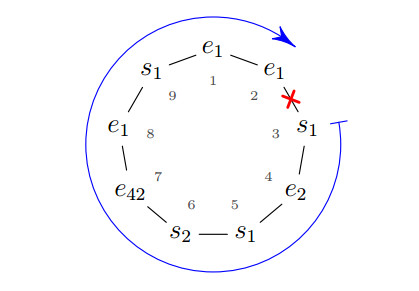
\includegraphics[scale=0.5]{DNA}\end{center}
	\caption{Illustration with its optimal cutting location.}	
	\label{DNA}
\end{figure}\\
{\bf Input}\\
The first line of input contains an integer n $(1 \leq n \leq 10^6)$, the length of the DNA. The next line
contains the DNA sequence, that is, n markers. Each marker is a character c followed by an integer i,
where $c \in {s, e}$ specifies whether it is a start or an end marker and i $(1 \leq i \leq 10^6)$ is the gene type of
the marker. The given DNA sequence has been obtained from the circular DNA by cutting at an arbitrary
location.
{\bf Output}\\
Output one line with two integers p and m, where p is the cutting position that maximizes the number
of different gene types that form a proper nesting, and m is this maximum number of gene types. The
DNA is cut just before the pth input marker (for instance, the cut shown in Figure \ref{DNA} has p = 3). If
more than one cutting position yields the same maximum value of m, output the smallest p that does so.

\subsection{Descripci\'on}
En un centro de investigaci\'on se est\'an estudiando cadenas de ADN. Una cadena simple de ADN est\'a compuesta por varios genes que se clasifican en distintos tipos identificados por un marcador(un entero i). Despu\'es de cierto trabajo de investigaci\'on, cada cadena de genes de tipo i se reduce a marcadores iniciales $s_i$ y finales $e_i$. Resulta de inter\'es determinar si los genes de tipo i est\'an apropiadamente anidados dentro de una cadena w, para ello se forma una nueva cadena considerando solo los marcadores de tipo i y dicha cadena debe tener una de las siguientes estructuras:\\
\begin{itemize}
	\item $s_ie_i$
	\item $s_iNe_i$, donde N es una cadena anidada apropiadamente
	\item $AB$, donde A y B son cadenas anidadas apropiadamente
	
\end{itemize}

Una complicaci\'on en la investigaci\'on es que se est\'an estudiando cadenas de ADN circulares(forman un ciclo cerrado) y para estudiarlas se necesita cortarlas en alg\'un punto. De esta manera las cadenas de un tipo de marcador estar\'an anidadas apropiadamente en dependencia de la posici\'on donde se realice el corte.\\

El problema consiste en encontrar una posici\'on para el corte que maximice la cantidad de tipos de marcadores anidados apropiadamente.\\

L\'imites\\
$N \leq 10^6$ es la longitud de la cadena\\
$1 \leq i \leq 10^6$ donde i son los tipos de marcadores\\
Tiempo L\'imite: 3 segundos\\

\subsection{Soluci\'on}
Si se logra identificar de manera eficiente para cada tipo de marcador i las posiciones donde se puede cortar la cadena y que el mismo est\'e anidado apropiadamente, entonces tendr\'iamos en total una cantidad lineal de intervalos de posiciones que al cortarlas provocan que un tipo de marcador este apropiadamente anidado. Siendo as\'i entonces el problema se reduce a encontrar la posici\'on que est\'e contenida en la mayor cantidad de intervalos.\\
Este problema en particular se puede resolver con una complejidad de O(|I| + N), donde I es el conjunto de intervalos y N la cantidad de posiciones.\\ 
Definici\'on: ${AA}_i$ es una arreglo acumulativo construido a partir de $A_i$ si y solo si ${AA}_i = \sum_{j=0}^{i} A_j$\\
El algoritmo requiere construir un arreglo acumulativo a partir de otro arreglo A que se construye de la siguiente manera:\\
\begin{algorithm}
	{\bf Para Cada}$\;1 \leq j \leq N$ {\bf Hacer}\\ 
     \hspace{1cm}$ A_j = 0$\\
	{\bf Fin Para} \\
	{\bf Para Cada} $[l_j, r_j] \in \; I$ {\bf Hacer}\\
	\hspace{1cm}$A_{lj} = A_{lj} + 1$\\
	\hspace{1cm}$A_{rj + 1} = A_{rj + 1} - 1$\\
	{\bf Fin Para} \\
\end{algorithm}\\
Una vez construido el arreglo acumulativo de A, el valor de cada posici\'on representa la cantidad de intervalos que contienen dicha posici\'on. N\'otese que $AA_k$ = Cantidad de intervalos que comienzan en una posici\'on $\leq k$ menos la cantidad de intervalos que terminan en una posici\'on $<k$, lo que es en esencia
la cantidad de intervalos que contienen la posici\'on k. Con ese resultado simplemente nos quedamos con el mayor valor y queda resuelto el problema.\\

Ahora queda encontrar de manera eficiente los intervalos de posiciones donde se puede cortar una cadena circular de un tipo de marcador i y que esta muestre un anidamiento apropiado. 	
De la definici\'on recursiva se puede observar que para cada marcador inicial debe existir uno final, de aqu\'i la soluci\'on a este subproblema comienza por ignorar un tipo de marcador i si las cantidades de $s_i$ y $e_i$ difieren, ya que este nunca estar\'a anidado apropiadamente. A partir de ahora solo se considerar\'an cadenas con iguales cantidades de $s_i$ y $e_i$.\\
Ejemplos de cadenas anidadas apropiadamente: $s_i \; s_i \; e_i \; e_i $,\hspace{1cm}$s_i \; e_i \; s_i \; e_i$,\hspace{1cm}$s_i \; s_i \; e_i \; s_i \; e_i \; e_i$.\\
Ejemplos de cadenas no anidadas apropiadamente: $e_i \; s_i $,\hspace{1cm}$s_i \; e_i \; e_i \; s_i$.\\

Se puede observar adem\'as que a cada elemento de fin le corresponde el elemento de inicio m\'as pr\'oximo a la izquierda que no se haya emparejado ya. Si para un elemento de fin no existe uno de inicio correspondiente entonces la cadena no est\'a anidada apropiadamente.
Este hecho sugiere un algoritmo sencillo con una pila para comprobar si una cadena est\'a apropiadamente anidada o no. Esta estructura se puede contemplar como un lenguaje libre de contexto y como consecuencia se puede reconocer cadenas que pertenecen a dicho lenguaje con un aut\'omata de pila\cite{Gramatica1}\cite{Gramatica2}.Recorremos la cadena de izquierda a derecha y consideramos dos casos: si encontramos un elemento de inicio lo ponemos en la pila y en caso de ser un elemento de fin lo emparejamos con el del tope de la pila. Si en alg\'un momento se encuentra un elemento de fin y la pila est\'a vac\'ia entonces la cadena no est\'a anidada apropiadamente. En este caso donde solo se necesita comprobar y los elementos de inicio son indistinguibles se puede simplemente almacenar el tama\~no actual de la pila en una variable entera. Veamos esta variable entera como un contador que se incrementa con cada $s_i$ y se decrementa con cada $e_i$, si al final de la cadena el contador tuvo valor menor que cero en alguna posici\'on  entonces la cadena no est\'a anidada apropiadamente.\\
Como estamos en presencia de cadenas circulares se deben considerar todas las cadenas posibles obtenidas por un corte. Suponiendo que tenemos una cadena de tama\~no n una t\'ecnica eficiente para esto es duplicar la cadena y analizar todas las subcadenas de tama\~no n.\\
Ahora consideremos una cadena S de un tipo de marcador determinado, luego obtenemos S+S(concatenaci\'on de S consigo misma) y aplicamos el algoritmo descrito arriba almacenando para cada posici\'on j de S+S el valor del contador hasta ese momento. Luego para cada subcadena de tama\~no n, digamos desde la posici\'on j hasta j+n-1 comprobamos que el m\'inimo valor del contador en ese intervalo es 0. Si es as\'i entonces es una subcadena anidada apropiadamente y tenemos un posible corte. Hay que tener en cuenta adem\'as que para simular que se comenz\'o a contar desde la posici\'on j se debe restar el valor que ten\'ia el contador en la posici\'on j-1.\\
Para obtener el m\'inimo valor en un intervalo de manera eficiente se puede usar alguna estructura de datos como Segment Tree o Range Minimum Query\cite{Halim}\cite{SegmentTree}.\\
La soluci\'on del primer subproblema explicado posee complejidad O(N) ya que $|I|$ es a lo m\'as N. Mientras que en el segundo subproblema el uso de las estructuras de datos permite obtener el m\'inimo de un intervalo en O(log N), este proceso se realiza N veces en total por lo que se tiene una complejidad O(N log N). Por lo tanto se concluye que la complejidad total del programa es O(N log N). Una observaci\'on adicional es la siguiente: Para obtener los valores reales del contador en un intervalo [j , j+n-1] se debe restar el valor en la posici\'on j-1 como se mencion\'o anteriormente, esto indica que si ese valor es mayor que alg\'un valor del arreglo entonces al restarlo se obtendr\'ia un valor menor que 0. Por tanto dicha posici\'on j-1 para el corte debe poseer el menor valor del arreglo (pueden ser varias posiciones), y se pueden identificar directamente en O(N). Con esta \'ultima observaci\'on en el peor caso se realizan $4\cdot 10^6$ operaciones, menor que las $3 \cdot 10^8$ permisibles seg\'un el l\'imite de tiempo establecido para el problema. La soluci\'on tiene complejidad espacial $O(N)$, en el peor caso almacena $10^6 \cdot 4\; bytes$, menor que los $10^9 \;bytes$ permitidos.
\subsection{C\'odigo}
\begin{lstlisting}[language=C++]
#include<bits/stdc++.h>
using namespace std;

typedef pair<int,int>par;
const int MAXN=1e6+5;

int getMarker(string in)
{
	int ret=0;
	for(int i=1; i<in.size(); i++)
	{
		ret*=10;
		ret+=(in[i]-'0');
	}
	return ret;
}

set<int>M;
vector<par>V[MAXN];
int C[MAXN];
int TA[MAXN];


int main()
{
	cin.tie(0);
	ios_base::sync_with_stdio(0);

	int N;
	cin >> N;

	string in;
	for(int i=1; i<=N; i++)
	{
		cin >> in;
		char c=in[0];
		int marker=getMarker(in);
		if(c=='s')
			V[marker].push_back(par(1,i)),C[marker]++;
		else
			V[marker].push_back(par(-1,i)),C[marker]--;

		M.insert(marker);
	}

	multiset<par>I;

	for(auto i:M)
	{
		if(C[i])continue;
		int c=0;
		int minc=1<<30;
		for(auto p:V[i])
		{
			c+=p.first;
			minc=min(minc,c);
		}
		c=0;
		for(int j=0; j<V[i].size(); j++)
		{
			c+=V[i][j].first;
			if(c==minc && j+1<V[i].size())
				I.insert(par(V[i][j].second+1,V[i][j+1].second));
			else if(c==minc)
			{
				if(V[i][j].second+1<=N)
				I.insert(par(V[i][j].second+1,N));
				I.insert(par(1,V[i][0].second));
			}
		}
	}

	for(auto p:I)
	{
		TA[p.first]++;
		TA[p.second+1]--;
	}

	int solV=0,solP=1;
	for(int i=1; i<=N; i++)
	{
		TA[i]+=TA[i-1];
		if(TA[i]>solV)
		{
			solV=TA[i];
			solP=i;
		}
	}

	cout << solP << ' ' << solV << '\n';

	return 0;
}
\end{lstlisting}

\section{Problema E. Dead-End Detector}
The council of your home town has decided to improve road sign placement,
especially for dead ends. They have given you a road map, and you must
determine where to put up signs to mark the dead ends. They want you to
use as few signs as possible.
The road map is a collection of locations connected by two-way streets. The
following rule describes how to obtain a complete placement of dead-end
signs. Consider a street S connecting a location x with another location. The
x-entrance of S gets a dead-end sign if, after entering S from x, it is not
possible to come back to x without making a U-turn. A U-turn is a 180-
degree turn immediately reversing the direction.
To save costs, you have decided not to install redundant dead-end signs, as specified by the following
rule. Consider a street S with a dead-end sign at its x-entrance and another street T with a dead-end
sign at its y-entrance. If, after entering S from x, it is possible to go to y and enter T without making a
U-turn, the dead-end sign at the y-entrance of T is redundant. See Figure \ref{DeadEnd}for examples.
\begin{figure}[h]
	\begin{center}
\includegraphics[scale=0.45]{DeadEnd}\end{center}
	\caption{Illustration indicating where non-redundant dead-end signs
		are placed.}	
	\label{DeadEnd}
\end{figure}\\
{\bf Input}\\
The first line of input contains two integers n and m, where n $(1 \leq n \leq 5 \cdot 10^5)$ is the number of
locations and m $(0 \leq m \leq 5 \cdot 10^5)$ is the number of streets. Each of the following m lines contains two
integers v and w $(1 \leq v < w \leq n)$ indicating that there is a two-way street connecting locations v and
w. All location pairs in the input are distinct.\\
{\bf Output}\\
On the first line, output k, the number of dead-end signs installed. On each of the next k lines, output two
integers v and w marking that a dead-end sign should be installed at the v-entrance of a street connecting
locations v and w. The lines describing dead-end signs must be sorted in ascending order ofv-locations,
breaking ties in ascending order of w-locations.

\subsection{Descripci\'on}
En el problema b\'asicamente describen una ciudad con varias localidades y calles que las conectan. Se nos pide colocar de manera correcta ciertas se\~nales de calle sin salida, pero adem\'as identificar las se\~nales redundantes para ahorrar recursos evitando colocarlas.
Es el t\'ipico problema que podemos modelar como un grafo, no orientado en este caso, donde las localidades ser\'ian los nodos y las calles las aristas.\\
Una se\~nal de calle sin salida la podemos ver como una relaci\'on CSS(v,e) donde v es un nodo y e es una arista.\\
De manera formal sea V el conjunto de nodos y E el conjunto de aristas:\\
 CSS(v,e),$\ v \in V,e \in E$ si despu\'es de entrar en e por v no es posible volver a v sin hacer un giro en U.\\
Con respecto a la redundancia de las se\~nales:\\
CSS(v,e),$\ v \in V,e \in E$ es redundante si existe $v1 \in V$ y $e1 \in E$ tal que CSS(v1,e1) y despu\'es de entrar a e1 por v1 se puede llegar a e entrando por v.\\

L\'imites\\
$|V| \leq 5\cdot10^5$\\
$|E| \leq 5\cdot10^5$\\
Tiempo L\'imite: 5 segundos\\

\subsection{Soluci\'on}
La primera observaci\'on es que cada componente conexa del grafo se puede analizar de manera independiente. Para abordar la soluci\'on de este problema debemos considerar dos casos: caso de que la componente conexa sea un \'arbol y el caso de que tenga al menos un ciclo.\\
Caso de un \'arbol:\\
{\bf Proposici\'on}: En un \'arbol todas las aristas tienen se\~nal de calle sin salida en ambos extremos.\\
{\bf Demostraci\'on}:\\
Sea $v \in V$ y $e \in E$ una arista incidente en v, al entrar en e por v se llega a otro nodo u donde existen dos opciones. La primera es volver inmediatamente a v, donde estar\'iamos haciendo un giro en U por lo que no es posible. La segunda ser\'ia recorrer un camino hasta un nodo w del \'arbol y regresar al nodo u sin hacer un giro en U para luego ir a v, esta segunda opci\'on tampoco es posible porque como estamos en presencia de un \'arbol para todo nodo w existe un \'unico camino entre u y w por lo que necesariamente estar\'iamos haciendo un giro en U para volver. Por lo anterior queda demostrado que no es posible regresar a v sin hacer un giro en U y existe la relaci\'on CSS(v,e).\\
{\bf Proposici\'on}: CSS(v,e) es redundante ssi v no es un nodo colgante\\
{\bf Demostraci\'on}:Hay dos proposiciones que demostrar aqu\'i, la primera es que si CSS(v,e) es redundante entonces v tiene grado mayor que 1. Por la definici\'on de redundancia se sabe que existe $v1 \in V$ y $e1 \in E$ tal que CSS(v1,e1) y luego de entrar en e1 por v1 existe un camino hasta v que no contiene a e. Lo anteriormente planteado indica que v debe tener grado al menos 2 por lo que no es un nodo colgante. La segunda proposici\'on dice que si v no es un nodo colgante entonces $\forall e \in E$ incidente en v se cumple CSS(v,e) es redundante. Para demostrar esto debemos considerar que si v no es colgante tiene grado al menos 2 y como se demostr\'o anteriormente todas las aristas en un \'arbol tienen una se\~nal en ambos extremos. Con estos hechos podemos decir que $\forall u \in V$ tal que exista la arista (v,u) tambi\'en existe una arista (w,v) con $w\in V $y $w \ne u$, ambas aristas tienen se\~nales en ambos extremos por lo que las se\~nales correspondientes a v son redundantes.\\
Con estas dos proposiciones se puede concluir que en el caso de un \'arbol pertenecen a la soluci\'on todas las aristas (v,u) con se\~nal en v si el grado de v es 1.\\
El otro caso a analizar en cuando la componente conexa tiene al menos un ciclo.\\ 
{\bf Proposici\'on}:\\
La arista (v,u) tiene una se\~nal de CSS en v ssi al quitarla se divide el grafo en dos componentes conexas y la componente que contiene a u es un \'arbol.\\
{\bf Demostraci\'on}:\\
Primero: La arista (v,u) tiene una se\~nal de CSS en v $=>$ al quitarla se divide el grafo en dos componentes conexas y la componente que contiene a u es un \'arbol. 
\\La demostraci\'on de esta afirmaci\'on se puede hacer por reducci\'on al absurdo. Supongamos que la arista (v,u) al quitarla no divide el grafo en dos componentes conexas, esto significa que existe un camino alternativo entre v y u que no contiene la arista (v,u) por lo que se pudiera volver a v sin hacer un giro en U y contradice la premisa. Por otro lado supongamos que si divide el grafo en dos componentes pero la componente que contiene a u no es un \'arbol, esto implica que en la componente de u existe al menos un ciclo y se podr\'ia desde u alcanzar el ciclo, recorrerlo y luego volver sin hacer un giro en U. El \'ultimo planteamiento tambi\'en contradice la premisa. Por tanto queda la primera proposici\'on demostrada.\\
Luego: Al quitar la arista (v,u) se divide el grafo en dos componentes conexas y la componente que contiene a u es un \'arbol $=>$ La arista (v,u) tiene una se\~nal de CSS en v. La premisa enunciada implica que no exista manera de regresar v (excepto por la arista (v,u)) luego de ir a u ya que la arista no es parte de un ciclo y en la componente de u al quitar la arista existe un \'unico camino entre cada par de nodos lo que hace imposible regresar sin hacer un giro en U como se hab\'ia analizado anteriormente.\\
Consideremos el siguiente algoritmo:\\
\begin{algorithm}[H] % H = forzar est\'a posici\'on
	\caption{EliminarSe\~nales(G)}\label{ML:Algorithm4}
	\SetAlgoLined
	\LinesNumbered
	\SetAlgoVlined
	{\bf Mientras} $\exists \;v\in G \;\backslash \;\; grado(v) = 1\;$ {\bf Hacer}\\
	\hspace{0,5cm} Eliminar v de G\\
	{\bf Fin Mientras}\\	
\end{algorithm}
\hspace{1cm}\\
{\bf Proposici\'on}:\\
El algoritmo elimina de G todas las aristas con se\~nal de CSS.\\
{\bf Demostraci\'on}:\\
Supongamos que el algoritmo termin\'o y qued\'o un arista (v,u) con una se\~nal en v que no fue eliminada, por lo demostrado anteriormente la arista (v,u) divide el grafo en dos componentes conexas y la correspondiente a u es un \'arbol. Esto indica que en la componente de u existe al menos un nodo colgante(grado = 1) y contradice que el algoritmo ya haya terminado.\\ 
{\bf Proposici\'on}:\\
El algoritmo no elimina de G aristas sin se\~nal de CSS.\\
{\bf Demostraci\'on}:\\
Si una arista no tiene se\~nalizaci\'on es porque es parte de un ciclo o divide el grafo en dos componentes pero ninguna de estas es un \'arbol. En el caso de que sea parte de un ciclo no puede ser eliminada ya que cada nodo en un ciclo est\'a conectado a al menos dos nodos en el ciclo. Por otro lado si la arista separa dos componentes conexas y ninguna de estas es un \'arbol entonces tienen al menos un ciclo que no podr\'a ser eliminado. Para eliminar la arista debe eliminarse con anterioridad una de las componentes lo cual es imposible por los ciclos que contienen cada una.\\
{\bf Proposici\'on}:\\
Una se\~nal de CSS en una arista entre dos nodos eliminados por el algoritmo es redundante.\\
{\bf Demostraci\'on}:\\
Sea u,v nodos eliminados por el algoritmo en ese orden, por lo demostrado la arista (v,u) tiene una se\~nal en v. Luego si v fue eliminado despu\'es de u entonces existe $w\ne u$ tal que la arista (w,v) tiene una se\~nal en w. De esta manera se demuestra que la se\~nal en (v,u) es redundante.\\
Por \'ultimo se concluye que las aristas parte de la soluci\'on son las que van de un nodo no eliminado a uno eliminado. La detecci\'on de las componentes conexas y el an\'alisis del primer caso se pueden realizar con una b\'usqueda en profundidad, complejidad O(N + M).
El algoritmo propuesto se puede implementar similar a una b\'usqueda a lo ancho comenzando con los nodos de grado 1, tambi\'en complejidad O(N + M). La complejidad algor\'itmica total de la soluci\'on es O(N + M). En el peor caso se realizan $2\cdot 10^6$ operaciones, menor que las $5 \cdot 10^8$ permisibles seg\'un el l\'imite de tiempo establecido para el problema. La soluci\'on tiene complejidad espacial $O(N + M)$, en el peor caso almacena $10^6 \cdot 4\; bytes$, menor que los $10^9 \;bytes$ permitidos.\\

\subsection{C\'odigo}
\begin{lstlisting}[language=C++]
#include<bits/stdc++.h>
using namespace std;

typedef pair<int,int>par;
const int MAXN=5e5+5;
vector<int>ady[MAXN];
typedef pair<int,int>par;


int CC[MAXN];
int CN[MAXN];
bool notTree[MAXN];
int cc;
par E[MAXN];
int G[MAXN];
bool Eliminado[MAXN];

void dfs(int nod,int parent=-1)
{
	CC[nod]=cc;
	CN[cc]++;
	for(auto nn:ady[nod])
	{
		if(CC[nn])
		{
			if(nn!=parent)
			notTree[cc]=true;
			continue;
		}
		dfs(nn,nod);
	}
}

int main()
{
	cin.tie(0);
	ios_base::sync_with_stdio(0);
	
	int N,M;
	cin >> N >> M;
	
	int a,b;
	for(int i=1; i<=M; i++)
	{
		cin >> a >> b;
		ady[a].push_back(b);
		ady[b].push_back(a);
		E[i]=par(a,b);
		G[a]++,G[b]++;
	}
	
	for(int i=1; i<=N; i++)
	{
		if(CC[i])continue;
		cc++;
		dfs(i);
	}
	
	queue<int>cola;
	vector<par>sol;
	
	for(int i=1; i<=M; i++)
	{
		int a=E[i].first;
		int b=E[i].second;
		if(notTree[CC[a]])
		{
			if(G[a]==1)
			cola.push(a);
			if(G[b]==1)
			cola.push(b);
		}
		else
		{
			if(G[a]==1)
			sol.push_back(par(a,b));
			if(G[b]==1)
			sol.push_back(par(b,a));
		}
	}
	
	while(!cola.empty())
	{
		int nod=cola.front();
		Eliminado[nod]=true;
		cola.pop();
		
		for(auto nn:ady[nod])
		{
			if(Eliminado[nn])continue;
			G[nn]--;
			if(G[nn]==1)
			cola.push(nn);
		}
	}
	
	for(int i=1; i<=M; i++)
	{
		int a=E[i].first;
		int b=E[i].second;
		if(Eliminado[a] && !Eliminado[b])
		sol.push_back(par(b,a));
		if(Eliminado[b] && !Eliminado[a])
		sol.push_back(par(a,b));
	}
	
	sort(sol.begin(),sol.end());
	cout << sol.size() << '\n';
	for(auto i:sol)
	cout << i.first << ' ' << i.second << '\n';
	
	
	
	
	return 0;
}
\end{lstlisting}
\section{Problema G. First of Her Name}
In the Royal Family, names are very important! As the Royal Historian you have been charged with
analyzing the patterns in the names of the Royal Ladies in the realm.
There have been n Royal Ladies, for convenience numbered from 1 to n. The name of each Lady is an
uppercase letter concatenated with the name of her mother. The exception is the Lady numbered 1, the
founder of the Royal Family, whose name is just a single uppercase letter.
For example, ENERYS could be the mother of AENERYS (as the name AENERYS consists of the single
uppercase letter 'A' concatenated with ENERYS, which is her mother's name). Similarly, AENERYS
could be the mother of DAENERYS and YAENERYS.
You are given the description of all the Royal Ladies. Your task is to determine, for certain interesting
strings s, the number of Royal Ladies for whom s is a prefix of their name.
For example, consider Sample Input 1 below, with a Royal Line that goes straight from the founder S
to AENERYS (through YS, RYS, ERYS, NERYS and ENERYS), with each Lady having exactly one
daughter. Then AENERYS has two daughters-DAENERYS and YAENERYS, with the latter having
one daughter, RYAENERYS.
In such a family, RY is a prefix of the names of two ladies: RYS and RYAENERYS. E is a prefix of the
names of ERYS and ENERYS. N is a prefix only of NERYS's name, while S is a prefix only of the name
of the founder, S. AY is not a prefix of any Royal Lady's name.\\
{\bf Input}\\
The first line of input contains two integers n and k, where n $(1 \leq n \leq 10^6)$ is the total number of Royal
Ladies and k $(1 \leq k \leq 10^6)$ is the number of query strings.
Then follow n lines describing the Royal Ladies. The ith of these lines describes the Royal Lady numbered i, and contains an uppercase letter $c_i$ ('A'-'Z') and an integer $p_i$, where $c_i$ is the first letter of the
name of Lady i, and $p_i$ ($p_1$ = 0 and $1 \leq p_i < i$ for i > 1) is the number of her mother (or 0, in the case
of the First Lady). All the names are unique.
The remaining k lines each contain one nonempty query string, consisting only of uppercase letters. The
sum of the lengths of the query strings is at most $10^6$.\\
{\bf Output}\\
Output k lines, with the ith line containing the number of Royal Ladies who have the ith query string as
a prefix of their name.

\subsection{Descripci\'on}
En el problema nos describen como se forman los nombres de las se\~noras de la realeza, b\'asicamente definen que el nombre de una se\~nora se forma escogiendo una letra may\'uscula y concaten\'andole por la derecha el nombre de su madre. Nos dicen que se conocen N se\~noras reales numeradas convenientemente de 1 a N, de cada una se conoce la letra escogida para su nombre y quien es su madre entre las restantes, excepto para la n\'umero 1 cuyo nombre es una simple letra.
Dada la informaci\'on anteriormente descrita se nos pide responder Q preguntas de la forma siguiente: para una cadena S cu\'antos nombres de se\~noras contienen a S como prefijo.\\
L\'imites\\
$N \leq 10^6$\\
$Q \leq 10^6$\\
la suma de las longitudes de las cadenas preguntadas no excede $10^6$\\
Tiempo L\'imite: 10 segundos\\

\subsection{Soluci\'on}
Una soluci\'on trivial para este problema ser\'ia construir los nombres de las N se\~noras y luego recorrerlos por cada pregunta comprobando lo pedido. Esta idea no satisface los l\'imites de tiempo ni de espacio. Una mejora ser\'ia ordenar los nombres, de esta manera el conjunto que contienen la cadena de la pregunta como prefijo forman un intervalo que se puede identificar con b\'usqueda binaria. As\'i la respuesta a las preguntas se realiza en O(L log N) donde L es la longitud total de las preguntas. A\'un as\'i construir todos los nombres resulta imposible por cuesti\'on de espacio, adem\'as ordenarlos de la manera est\'andar ser\'ia en O($N^2\;log\;N$) ya que el ordenamiento es en O(N log N) y la comparaci\'on de dos nombres es en O(N), esto es demasiado lento. Una soluci\'on para ambas situaciones es ordenar usando la idea del Suffix Array, este se basa en mantener en orden de los sufijos por sus prefijos de tama\~no $2^k$ en el kth paso\cite{SuffixArray}. Con esta idea se pueden ordenar todos los \'indices sin necesidad de construir los nombres y el ordenamiento quedar\'ia en O(N $log^2$ N) o O(N log N) si se usa Counting Sort. Para implementar el algoritmo es necesario calcular en O(1) el $2^k$th caracter de un nombre determinado, esto se puede lograr precalculando una tabla de la forma $T[i][k]$ indicando la posici\'on $2^k$ del nombre que comienza en el \'indice i. Este prec\'alculo se puede realizar con programaci\'on din\'amica, los casos bases ser\'ian $T[i][0]$ ya conocido y la recurrencia $T[i][k]=T[ T[i][k-1] ][k-1]$. En el peor caso se realizan $4\cdot 10^8$ operaciones, menor que las $10 \cdot 10^8$ permisibles seg\'un el l\'imite de tiempo establecido para el problema. La soluci\'on tiene complejidad espacial $O(N \;log\;N)$, en el peor caso almacena $20\cdot 10^6 \cdot 4\; bytes$, menor que los $10^9 \;bytes$ permitidos.

\subsection{C\'odigo}
\begin{lstlisting}[language=C++]
#include <bits/stdc++.h>
using namespace std;

const int MAXN=2e6+5;

struct T
{
    int nr[2],p;
} L[MAXN];

bool com(const T &s,const T &p)
{
    if(s.nr[0]!=p.nr[0])
        return s.nr[0]<p.nr[0];

    return s.nr[1]<p.nr[1];
}

int N,K,stp,delta;
char S[MAXN];
int P[25][MAXN];
int Pos[MAXN];
int Nxt[MAXN][25];
int Len[MAXN];

bool MayorIgual(int p,string &aux)
{
    p=Pos[p];
    int p1=0;
    int sz=aux.size();

    while(p!=-1 && p1<sz && S[p]==aux[p1])
    {
        p1++;
        p=Nxt[p][0];
    }
    if(p==-1 && p1<sz)
        return false;

    if(p1<sz && S[p]<aux[p1])
        return false;

    return true;
}

bool MenorIgual(int p,string &aux)
{
    p=Pos[p];
    int p1=0;
    int sz=aux.size();

    while(p!=-1 && p1<sz && S[p]==aux[p1])
    {
        p1++;
        p=Nxt[p][0];
    }

    if(p!=-1 && p1<sz && S[p]>aux[p1])
        return false;

    return true;
}

int main()
{
    cin.tie(0);
    ios_base::sync_with_stdio(0);

    int N,Q;
    cin >> N >> Q;

    memset(Nxt,-1,sizeof Nxt);

    for(int i=0; i<N; i++)
    {
        cin >> S[i] >> Nxt[i][0];
        Nxt[i][0]--;
    }

    for(int stp=1; (1<<stp)<=N; stp++)
    {
        for(int i=0; i<N; i++)
            Nxt[i][stp]=Nxt[Nxt[i][stp-1]][stp-1];
    }
    Len[0]=1;
    for(int i=1; i<N; i++)
    {
        int stp=0;
        while(Nxt[i][stp]!=-1)
            Len[i]=1<<stp,stp++;
    }

    for(int i=0; i<N; i++)
        P[0][i]=S[i]-'A';

    for(stp=1,delta=1; (delta>>1) < N; stp++,delta<<=1)
    {
        for(int i=0; i<N; i++)
        {
            L[i].nr[0]=P[stp - 1][i];
            L[i].p = i;
            if(Nxt[i][stp-1]!=-1)
                L[i].nr[1]=P[stp-1][Nxt[i][stp-1]];
            else
                L[i].nr[1]=-(i+1);
        }
        sort(L,L+N,com);

        for(int i=0; i<N; i++)
        {
            if(i>0 && L[i].nr[0] == L[i - 1].nr[0] && L[i].nr[1] == L[i - 1].nr[1] )
                P[stp][L[i].p]=P[stp][L[i - 1].p];
            else
                P[stp][L[i].p]=i;
        }
    }

    for(int i=0; i<N; i++)
        Pos[P[stp-1][L[i].p]]=L[i].p;

    string aux;
    for(int i=0; i<Q; i++)
    {
        cin >> aux;

        //Lower Bound
        int lb=N-1;
        int I=0,F=N-1;
        while(I<=F)
        {
            int piv=(I+F)/2;
            if(MayorIgual(piv,aux))
                lb=piv,F=piv-1;
            else
                I=piv+1;
        }
        if(!MayorIgual(lb,aux))
            lb++;
        //Upper Bound
        int ub=lb-1;
        I=lb,F=N-1;
        while(I<=F)
        {
            int piv=(I+F)/2;
            if(MenorIgual(piv,aux))
                ub=piv,I=piv+1;
            else
                F=piv-1;
        }
        ub++;

        cout << ub-lb << '\n';
    }
    return 0;
}
\end{lstlisting}
\section{Problema H. Hobson's Train}
Mr. Hobson has retired from running a stable and has invested in a more modern form of transport,
trains. He has built a rail network with n stations. However, he has retained his commitment to free
the passenger from the burden of too many choices: from each station, a passenger can catch a train to
exactly one other station. Such a journey is referred to as a leg. Note that this is a one-way journey, and
it might not be possible to get back again.
Hobson also offers exactly one choice of ticket, which allows a passenger to travel up to k legs in one
trip. At the exit from each station is an automated ticket reader (only one, so that passengers do not need
to decide which to use). The reader checks that the distance from the initial station to the final station
does not exceed k legs.
Each ticket reader must be programmed with a list of valid starting stations, but the more memory this
list needs, the more expensive the machine will be. Help Hobson by determining, for each station A, the
number of stations (including A) from which a customer can reach A in at most k legs.
\begin{figure}[h]
	\begin{center}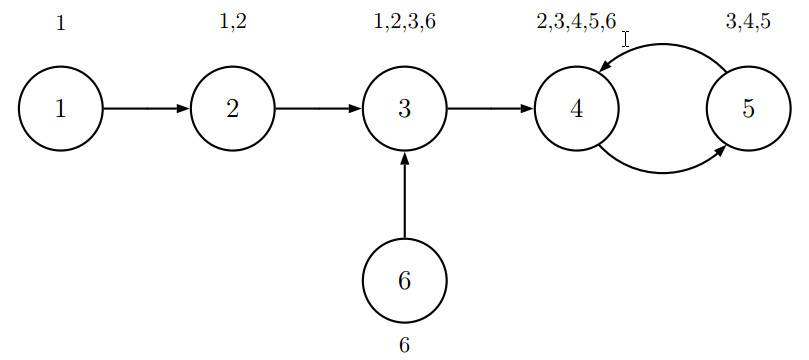
\includegraphics[scale=0.45]{Train}\end{center}
	\caption{Each circle represents a station. The numbers
		outside the circles are the station numbers loaded into the ticket readers when k = 2.}	
	\label{Train}
\end{figure}\\
{\bf Input}\\
The first line of input contains two integers n and k, where n $(2 leq n \leq 5 · 10^5)$ is the number of stations
and k $(1 \leq k \leq n − 1)$ is the maximum number of legs that may be traveled on a ticket. Then follow n
lines, the ith of which contains an integer $d_i\; (1 \leq d_i \leq n \;and\; d_i \ne i)$, the station which may be reached
from station i in one leg.\\
{\bf Output}\\
Output n lines, with the ith line containing the number of stations from which station i can be reached
in at most k legs.\\
\subsection{Descripci\'on}
En el problema nos describen una red de estaciones de trenes, aclara que desde cada estaci\'on solo es posible viajar a exactamente otra estaci\'on. Llam\'emosle viaje a la acci\'on de tomar un tren desde una estaci\'on a la siguiente, el problema nos pide calcular para cada estaci\'on $i$ cu\'antas estaciones $j$ existen tal que es posible llegar desde $j$ a $i$ realizando K viajes o menos.\\
L\'imites\\
$N \leq 5\cdot10^5$ estaciones\\
$K \leq N-1$\\
Tiempo L\'imite: 5 segundos\\

\subsection{Soluci\'on}
La estructura del grafo formado es conocida como grafo funcional, cada v\'ertice tiene grado de salida exactamente uno\cite{Skiena}. Si consideramos el grafo invertido tendremos un conjunto de ciclos con \'arboles colgando de los nodos pertenecientes a un ciclo. Esta estructura nos permite resolver el problema de manera separada para los nodos que pertenecen a un ciclo y para los que no. A partir de ahora si no se especifica nos estaremos refiriendo al grafo invertido.\\
Los ciclos pueden identificarse hallando las componentes fuertemente conexas dentro del grafo original. Otra manera de hacerlo es con una t\'ecnica conocida como la liebre y la tortuga, se basa en utilizar dos puntero, uno que se mueve un paso a la vez y otro dos pasos a la vez\footnote{\hyperlink{FloydAlgorithm}{https://en.m.wikipedia.org/wiki/Cycle\_detection}}. En ambos caso la complejidad algor\'itmica es O(N).\\
Cuando consideramos los nodo no pertenecientes a un ciclo podemos analizar el grafo como varios \'arboles con ra\'iz en un nodo de ciclo, para cada \'arbol resolvemos de manera independiente. Para cada nodo la respuesta ser\'ia la cantidad de nodos a distancia menor o igual que K en su sub\'arbol. De manera formal debemos calcular $f_i$ que es la cantidad de nodos en el sub\'arbol del nodo i a distancia menor o igual que K:\\
$\displaystyle f_i = (\sum_{j \;hijo \;de\; i}f_j - g_j ) + 1$ donde $g_j$ es la cantidad de nodos a distancia exactamente K\\
  Al sumar los $f_j$ para cada hijo j estamos contando la cantidad de nodos a distancia a lo m\'as K+1 y al restar $g_j$ estamos descontando los que est\'an a distancia K+1 exactamente por lo que obtenemos el valor deseado, se suma 1 por el propio nodo. El valor $g_i$ puede calcularse recorriendo el \'arbol con un DFS y para cada nodo actualizar el valor de su Kth antecesor, posiblemente llevando los antecesores en un arreglo que simule una pila. As\'i queda resuelto el problema para los nodos no parte de un ciclo. Todos los c\'alculos pueden realizarse con b\'usqueda en profundidad, O(N) en este caso.\\
Para los nodos parte de un ciclo debemos resolver de manera diferente. Un nodo de un ciclo es alcanzado por todos los nodos de su propio ciclo si el tama\~no del ciclo es menor o igual que K+1, en otro caso es alcanzado por K+1 nodos. Un nodo no parte de un ciclo alcanza en K pasos o menos a un intervalo continuo de nodos del ciclo en cuesti\'on, en caso de que alcance alguno. Un problema conocido y descrito en parte del problema D \ref{ProblemD} es, dado un conjunto de intervalos analizar para cada posici\'on en cu\'antos intervalos est\'a contenida, este problema se resuelve lineal y es equivalente a resolver para cada nodo de un ciclo cu\'antos nodos fuera del ciclo lo alcanzan. La complejidad total de la soluci\'on ser\'ia entonces O(N). En el peor caso realiza $10\cdot 10^5$ operaciones, menor que las $5 \cdot 10^8$ permisibles seg\'un el l\'imite de tiempo establecido para el problema. La soluci\'on tiene complejidad espacial $O(N)$, en el peor caso almacena $5\cdot 10^5 \cdot 4\; bytes$, menor que los $10^9 \;bytes$ permitidos. 
\subsection{C\'odigo}
\begin{lstlisting}[language=C++]
#include <bits/stdc++.h>
using namespace std;

const int MAXN=5e5+5;
vector<int>Prv[MAXN];
int MaxLevel;
int L[MAXN];
int Stack[MAXN],s;
int sol[MAXN],TA[MAXN];
int F[MAXN],Nxt[MAXN];
int N,K;

void dfs(int nod,int pad,int lv)
{
	L[lv]++;
	Stack[++s]=nod;
	MaxLevel=max(MaxLevel,lv);
	if(s-K>=1)
	F[Stack[s-K]]++;
	for(auto nn:Prv[nod])
	{
		if(nn==pad)continue;
		dfs(nn,nod,lv+1);
	}
	s--;
}

void g(int nod,int pad)
{
	sol[nod]=1;
	for(auto nn:Prv[nod])
	{
		if(nn==pad)continue;
		g(nn,nod);
		sol[nod]+=sol[nn]-F[nn];
	}
}
int main()
{
	cin.tie(0);
	ios_base::sync_with_stdio(0);
	
	cin >> N >> K;
	
	for(int i=1; i<=N; i++)
	{
		cin >> Nxt[i];
		Prv[Nxt[i]].push_back(i);
	}
	memset(sol,-1,sizeof sol);
	for(int nod=1; nod<=N; nod++)
	{
		if(sol[nod]!=-1)continue;
		
		int u,t;
		for (u = nod, t = Nxt[nod]; u != t && u != Nxt[t]; u = Nxt[u], t = Nxt[Nxt[t]]);
		vector<int> cycle;
		cycle.push_back(u);
		for (int i = Nxt[u]; i != u; i = Nxt[i])
		cycle.push_back(i);
		
		for(auto i: cycle)
		sol[i]=min(K+1,(int)cycle.size());
		
		int sz=cycle.size();
		for(int i=0; i<sz; i++)
		{
			for(auto j:Prv[cycle[i]])
			{
				if(i==0 && j==cycle[sz-1])continue;
				if(i>0 && j==cycle[i-1])continue;
				for(int k=1; k<=MaxLevel; k++)
				L[k]=0;
				MaxLevel=0,s=0;
				
				dfs(j,cycle[i],1);
				g(j,cycle[i]);
				
				for(int k=1; k<=MaxLevel; k++)
				{
					if(K<k)continue;
					
					if(K>=sz-1+k)
					TA[0]+=L[k];
					else
					{
						int r=i+K-k;
						TA[i]+=L[k];
						if(r>=sz)
						{
							r=r%sz;
							TA[0]+=L[k];
							TA[r+1]-=L[k];
						}
						else if(r+1!=sz) TA[r+1]-=L[k];
					}
				}
			}
		}
		for(int k=0; k<sz; k++)
		{
			TA[k]+=TA[k-1];
			sol[cycle[k]]+=TA[k];
		}
		for(int k=0; k<sz; k++)
		TA[k]=0;
	}
	
	for(int i=1; i<=N; i++)
	cout << sol[i] << '\n';
	
	return 0;
}
\end{lstlisting}

\chapter*{Conclusiones}
\label{chap:Conclusiones}
\addcontentsline{toc}{chapter}{Conclusiones}

En el presente trabajo se le dio soluci\'on a 6 de los problemas de la Final Mundial del ICPC 2019. Como parte del an\'alisis de estas soluciones se demostraron las proposiciones empleadas y se calcul\'o la complejidad computacional de cada una. Por \'ultimo se implementaron de manera correcta cada una de las soluciones planteadas, los c\'odigos fueron aceptados en el juez online Kattis donde se encuentran disponibles los problemas de la Final Mundial \hyperlink{Kattis}{https://icpc.kattis.com/problems}. De esta manera concluimos en que se han cumplido los objetivos trazados para el trabajo en cuesti\'on. \\

\chapter*{Recomendaciones}
\label{chap:Recomendaciones}
\addcontentsline{toc}{chapter}{Recomendaciones}

Se recomienda garantizar la disponibilidad de trabajos como el presente en entornos virtuales que permitan el acceso de los estudiantes de la carrera Ciencia de la Computaci\'on. Por otro lado se recomienda la orientaci\'on de los estudiantes en el uso de jurados en l\'inea donde puedan enviar sus propias soluciones y compararlas con las propuestas anteriormente. Por \'ultimo, fomentar la participaci\'on de los estudiantes en un curso optativo de programaci\'on competitiva. 


\renewcommand{\bibname}{Referencia Bibliogr\'afica}
\bibliographystyle{plain}
\addcontentsline{toc}{chapter}{Referencia Bibliogr\'afica}

\begin{thebibliography}{9}

\bibitem{Cormen}
Cormen, T.H. (2009) Introduction to algorithms. MIT press.

\bibitem{Halim}
Halim, S., Halim, F., Skiena, S.S., \& Revilla, M.A. (2013). Competitive Programming 3. Lulu Independent Publish.

\bibitem{Knuth}
Knuth, D.E. (1997). Art of computer programming: sorting and searching (Vol. 3). Pearson Education.

\bibitem{TextAlgorithm}
Crochemore, M., \& Rytter, W. (1994). Text algorithms. Maxime Crochemore. 

\bibitem{Aurora}
Gil, A. (2018). An\'alisis de soluciones de problemas seleccionados de la Final Mundial del ICPC 2018.

\bibitem{SuffixArray}
Vladu, A., \& Negruseri, C. (2005). Suffix arrays-a programming contest approach.

\bibitem{SuffixArray1}
Karkkainen, J., \& Sanders, P. (2003, June). Simple linear work suffix array construction. In International Colloquium on Automata, Languages, and Programming (pp. 943-955). Springer, Berlin, Heidelberg.

\bibitem{Skiena}
Pemmaraju, S., \& Skiena, S. (2003). Computational Discrete Mathematics: Combinatorics and Graph Theory with Mathematica. Cambridge university press.

\bibitem{Graph1}
Deo, N. (2017). Graph theory with applications to engineering and computer science. Courier Dover Publications.

\bibitem{Graph2}
Trudeau, R. J. (2013). Introduction to graph theory. Courier Corporation.

\bibitem{DP1}
Hedetniemi, S., \& Goodman, S. (1977). Introduction to the Design and Analysis of Algorithms. McGraw-Hill, New York.

\bibitem{Gramatica1}
Ginsburg, S. (1966). The Mathematical Theory of Context Free Languages.[Mit Fig.]. McGraw-Hill Book Company.

\bibitem{Gramatica2}
Ginsburg, S., Greibach, S. A., \& Harrison, M. A. (1967). Stack automata and compiling. Journal of the ACM (JACM), 14(1), 172-201.

\bibitem{Complejidad1}
Papadimitriou, C. H. (2003). Computational complexity (pp. 260-265). John Wiley and Sons Ltd.

\bibitem{Complejidad2}
Alsuwaiyel, M. H. (2016). Algorithms: Design Techniques And Analysis (Revised Edition) (Vol. 14). World Scientific.

\bibitem{SegmentTree}
Setiadi, Iskandar. (2012). Segment Tree for Solving Range Minimum Query Problems. 10.13140/2.1.4279.2643.

\end{thebibliography}


\end{document}